\documentclass[aspectratio=169]{beamer}
\usetheme{WFCC}
\usepackage{booktabs}
\usepackage[backend=biber,style=authoryear,maxcitenames=2]{biblatex}
\addbibresource{references.bib}

\title[Research presentation]{Research presentation}
\subtitle{A portable dark Beamer theme}
\author[A. Researcher]{Alex Researcher}
\institute{Department / University}
\date{October 19, 2026}
\WFCCevent{Workshop or conference}
% Optional: use your own licensed image. Center-cropped to fill the right side.
% \WFCCtitleimage{assets/title-photo.jpg}
% \WFCCcollaborators{With collaborators at other institutions}

\begin{document}
\begin{frame}[plain]
  \titlepage
\end{frame}

\section{Motivation}
\begin{frame}{A clear research question}
  \begin{itemize}
    \setlength{\itemsep}{5mm}
    \item Introduce the question and why it matters.
    \item Describe the evidence the audience will see.
    \item Use \alert{emphasis} sparingly to highlight the key point.
  \end{itemize}
\end{frame}

\section{Methods}
\begin{frame}{Data and empirical approach}
  \begin{columns}[T,onlytextwidth]
    \begin{column}{.46\textwidth}
      \textbf{Data}\par\medskip
      Describe the sample, time period, unit of observation, and outcome.
      \medskip
      \begin{block}{Interpretation}
        Explain what variation identifies the parameter of interest.
      \end{block}
    \end{column}
    \begin{column}{.49\textwidth}
      \textbf{Model}
      \[
        y_{it}=\beta x_{it}+\alpha_i+\delta_t+\varepsilon_{it}
      \]
      \small Define the variables and distinguish the estimate from its identifying assumptions.
    \end{column}
  \end{columns}
\end{frame}

\section{Results}
\begin{frame}{An example table}
  \centering
  \begin{tabular}{lrr}
    \toprule
    Illustrative outcome & Estimate & Standard error\\
    \midrule
    Outcome A & $-0.12$ & 0.04\\
    Outcome B & $-0.08$ & 0.03\\
    Outcome C & $ 0.02$ & 0.02\\
    \bottomrule
  \end{tabular}
  \par\vspace{6mm}
  {\small\color{smokemuted}Invented numbers for layout demonstration only.}
\end{frame}

\begin{frame}{Figures and citations}
  \begin{columns}[c,onlytextwidth]
    \begin{column}{.48\textwidth}
      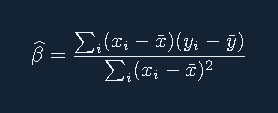
\includegraphics[width=\linewidth]{assets/example-figure.pdf}
    \end{column}
    \begin{column}{.47\textwidth}
      Keep figure text readable against the dark background.
      \par\medskip
      Example citation: \textcite{knuth1984texbook}.
      \par\medskip
      {\small\color{smokemuted}The figure at left is a typeset equation, included as a standalone PDF.}
    \end{column}
  \end{columns}
\end{frame}

\section{References}
\begin{frame}[allowframebreaks]{References}
  \small\printbibliography[heading=none]
\end{frame}
\end{document}
